\section{Experiments}
\label{Experiments}
\begin{figure}[t]
    \centering
    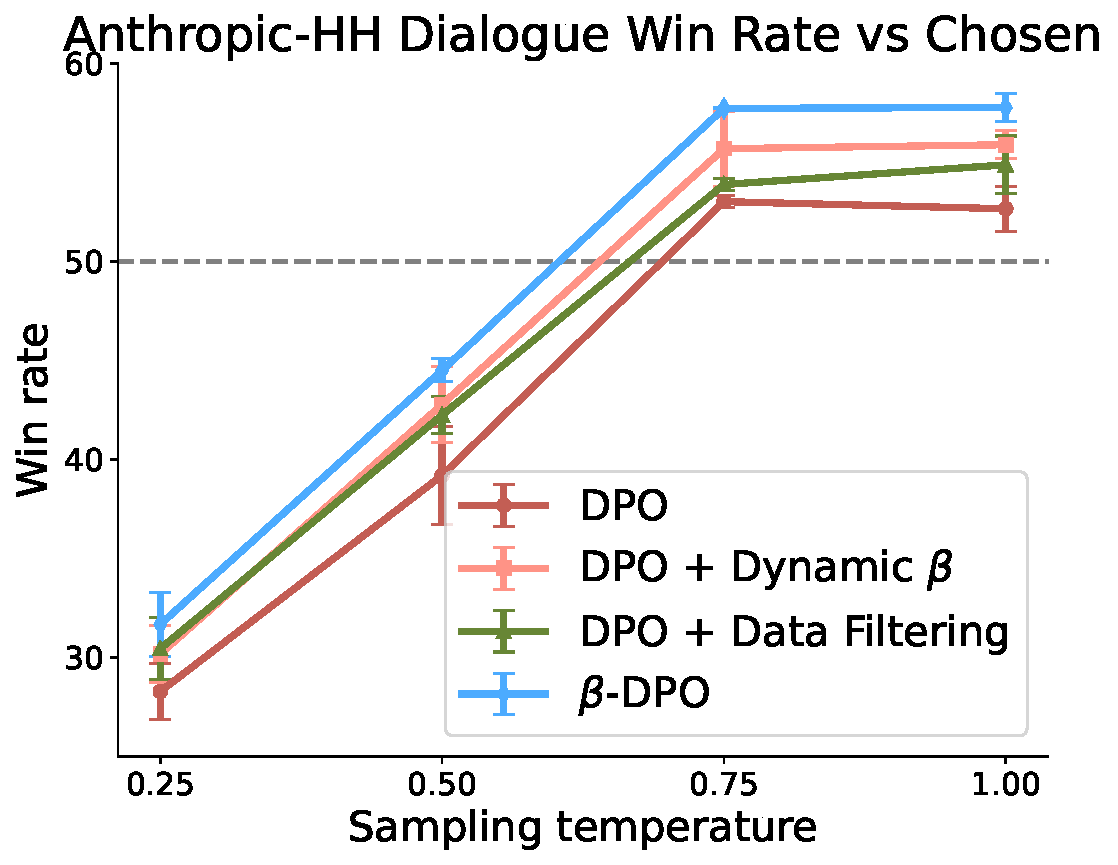
\includegraphics[width=0.49\textwidth]{figs/win_rate_hh.pdf}
    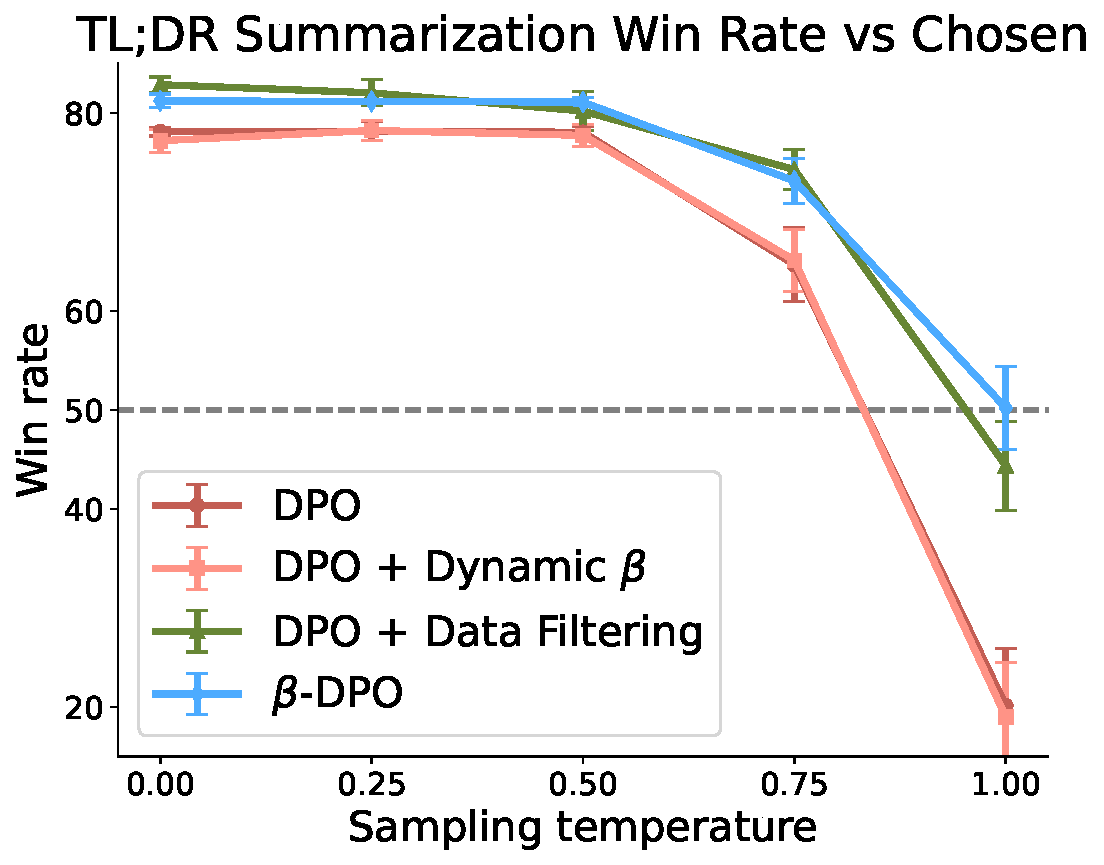
\includegraphics[width=0.49\textwidth]{figs/win_rate_tldr.pdf}
    \caption{
    \textbf{Left.} 
    The win rates computed by GPT-4 evaluations for the Anthropic-HH one-step dialogue; $\beta$-DPO consistently outperforms across all sampling temperatures.
    \textbf{Right.} 
    In the comparison of TL;DR summarization win rates versus chosen summaries with GPT-4 as the evaluator, $\beta$-DPO is distinguished as the only strategy achieving a win rate over 50\% across different sampling temperatures.
    }
    \label{fig:dialogue-main}
\end{figure}

In this section, we commence by conducting an empirical evaluation of $\beta$-DPO on two specific tasks: dialogue generation and summarization. Subsequently, we analyze the various adaptations of the proposed method $\beta$-DPO. Concluding this section, we underscore the imperative need for batch-level dynamic $\beta$ calibration, highlighting its significance in the context of our study.

\subsection{Empirical Evaluation of $\beta$-DPO on Dialogue Generation and Summarization}
\textbf{Datasets and Setup.} Our experiments are conducted on the Anthropic HH dataset \cite{Bai2022training} and Reddit TL;DR summarization dataset \cite{tldr_dataset}. The training configuration follows from \citet{DPO}. The goals of these experiments are to study: 1) How $\beta$-DPO performs on single-turn dialogue generation and summarization tasks; 2) How the sampling temperature affects the performance of $\beta$-DPO; 3) How $\beta$-DPO works with different model sizes. For detailed experimental settings, please refer to Appendix \ref{setup_exp}.

\textbf{Baselines.} In our comparison, we examine the performance of $\beta$-DPO relative to its counterparts: the standard DPO, DPO implemented with a dynamic $\beta$ yet devoid of $\beta$-guided data filtering, and DPO complemented by data filtering with $\beta$ fixed at 0.1.
% We compare $\beta$-DPO with DPO, DPO with dynamic $\beta$ (without $\beta$-guided data filtering), DPO with data filtering (keep $\beta$ as 0.1).

\textbf{Win Rate Across different Sampling Temperature.} An analysis of win rates derived from GPT-4 evaluations on the Anthropic-HH one-step dialogue demonstrates that $\beta$-DPO consistently outperforms across all sampling temperatures, as depicted in Figure \ref{fig:dialogue-main} (Left). Furthermore, for the TL;DR summarization task, $\beta$-DPO stands out as the only approach achieving win rates above 50\% for diverse sampling temperatures, which is visually represented in Figure \ref{fig:dialogue-main} (Right). The data also suggests that while both dynamic $\beta$ and data filtering enhance DPO's effectiveness, the impact of data filtering is especially pronounced in the summarization task, likely due to the inherently greater noise present in the Reddit TL;DR summarization dataset. Notably, $\beta$-DPO exhibits a remarkable degree of robustness to variations in sampling temperature. As the temperature incrementally escalates from 0.0 to 1.0, the win rate for standard DPO plunges to a mere 25\%, whereas $\beta$-DPO maintains a commendable performance level with a win rate of 54\%.

% \textbf{Win rate across different sampling temperature:} The win rates generated through GPT-4 evaluations for the Anthropic-HH one-step dialogue reveal that $\beta$-DPO consistently leads across all sampling temperature, as shown in Figure \ref{fig:dialogue-main} (left). On the TL;DR summarization task, $\beta$-DPO emerges as the sole methodology attaining a win rate exceeding 50\% across various sampling temperatures, as illustrated in Figure \ref{fig:dialogue-main} (right). In addition, we observe that dynamic $\beta$ and data filtering both can improve the performance of DPO, but data filtering is more significant in the summarization task. We attribute this to the fact that the Reddit TL;DR summarization dataset is more noisy than the Anthropic HH dataset. Moreover, we find $\beta$-DPO to be much more robust to the sampling temperatures, while sampling temperature increase from 0.0 to 1.0, DPO's win rate decreases to 25\%, while $\beta$ DPO still achieve 54\%.

\textbf{Win Rate Across Different Model Sizes.} We further evaluate the performance of $\beta$-DPO on the Anthropic HH dataset with Pythia-410M, -1.4B, and -2.8B models. The results are summarized in Table \ref{tab:ablation}. We observe that $\beta$-DPO consistently outperforms DPO, DPO with dynamic $\beta$, and DPO with data filtering across all model sizes.
We observe that in a smaller model, the improvement of data filtering is more significant, while in a larger model, the improvement of dynamic $\beta$ is more significant. We attribute this to the fact that the larger model has more capacity to learn the optimal policy, while the smaller model needs more help from the data filtering.



\begin{table}
    \centering
    \caption{
    % Win rate comparison on the Anthropic HH dataset with Pythia-410M, -1.4B, and -2.8B models. using GPT-4 as evaluator.
    Win rate comparison of Pythia-410M, -1.4B, and -2.8B models on the Anthropic HH dataset, evaluated using GPT-4.
    }
    \begin{tabular}{l|l|l|l}
        \toprule
        \textbf{Method} & \textbf{410M} & \textbf{1.4B} & \textbf{2.8B} \\
        \midrule
        DPO & $26.19$ & $42.78$ & $51.51$ \\
        DPO + Dynamic $\beta$ & $27.15^{\color{+}+ 3.67\%}$ & $43.51^{\color{+}+ 1.71\%}$ & $55.19^{\color{+}+ 7.14\%}$ \\
        DPO + Data Filtering & $29.03^{\color{+}+ 10.84\%}$ & $46.99^{\color{+}+ 9.84\%}$ & $53.42^{\color{+}+ 3.71\%}$ \\
        $\beta$-DPO & $30.18^{\color{+}+ 15.23\%}$ & $48.67^{\color{+}+ 13.77\%}$ & $57.07^{\color{+}+ 10.79\%}$ \\
        \bottomrule
    \end{tabular}
    \label{tab:ablation}
\end{table}




% We further investigate the performance of $\beta$-(IPO, KTO, SPPO) 
% In our work, we introduce a dynamic $\beta$ strategy, termed $\beta$-DPO, aimed at refining the decision process in the classical DPO framework and its variants: IPO, KTO, and SPPO. Our evaluation on the Anthropic HH dataset illustrates that, among the original variants, IPO outshines KTO and SPPO in terms of performance. By implementing our dynamic $\beta$ technique, creating dynamic versions: $\beta$-IPO, $\beta$-KTO, and $\beta$-SPPO, every variant witnesses a notable improvement in efficacy. Specifically, $\beta$-IPO demonstrates a significant performance leap of 17.9\%. This evidence solidly supports that the dynamic $\beta$ approach not only integrates seamlessly with existing DPO variants but also markedly propels their performance forward, offering a robust method for the advancement of language models trained with human feedback.

% \textbf{$\beta$-DPO adapts to and improves upon existing DPO's variants} 
% We further investigate the performance of $\beta$-(IPO, KTO, SPPO) across various DPO variants. As seen in Figure \ref{fig:gradient} (right),  it becomes apparent that neither KTO nor SPPO exhibits superiority over IPO when trained on the Anthropic HH dataset. Furthermore, our integration of the $\beta$ parameter into these models—IPO, KTO, SPPO—manages to enhance the performance of these DPO variants considerably. Notably, $\beta$-IPO registers a profound improvement of 17.9\%. These results strongly indicate that the $\beta$-augmented models—IPO, KTO, SPPO—constitute an adaptive and efficacious strategy for the development of language models trained via human feedback.
% KTO and SPPO is not superior to IPO on the Anthropic HH dataset. Besides, our $\beta$-(IPO, KTO, SPPO) still could improve the performance of these DPO variants, where $\beta$-IPO achieves significant 17.9\% improvement. This suggests that $\beta$-(IPO, KTO, SPPO) is a adaptive and effective method for training language models with human feedback. 
% \begin{table}
%     \centering
%     \caption{Ablation study of $\beta$-DPO on the Anthropic HH dataset using GPT-4 as evaluator.}
%     \begin{tabular}{l|l}
%         \toprule
%         \textbf{Method} & \textbf{Win Rate} \\
%         \midrule
%         IPO & $52.05$ \\
%         $\beta$-IPO & $54.73^{\color{+}+ 5.15\%}$ \\
%         \midrule
%         ORPO & $36.11$ \\
%         $\beta$-ORPO & $38.60^{\color{+}+ 6.90\%}$ \\
%         \bottomrule
%     \end{tabular}
%     \label{tab:ipo_orpo}
% \end{table}





\subsection{Adaptations of $\beta$-DPO}
\label{exp_adaptation}
In this section, our inquiry is twofold: first, we aim to understand the performance of $\beta$-DPO when applied across various filtering strategies; second, we examine its efficacy across different adaptations of the DPO framework. In terms of filtering strategies, prevailing studies \cite{pruthi2020estimating, xia2024less} in the domain largely employ a gradient-based approach. We propose to extend this methodology into three distinct scenarios. This involves arranging the gradients of pairwise data within a batch and consequently: (1) Excluding the top 20\% of samples, hereby referred to as \textbf{Filter Head},
(2) Excluding the bottom 20\% of samples, hereby referred to as \textbf{Filter Tail},
(3) Excluding both the top and bottom 10\% of samples, a method we denote as \textbf{Filter Tail \& Head}.
For a fair comparison, we maintain the amount of data excluded at 20\% for the above strategies.
Second, we integrate three variants of DPO into our analysis: the IPO \cite{ipo}, a novel approach that facilitates learning directly from preferences without the need for the Bradley-Terry (BT) model. Additionally, we consider the KTO \cite{KTO}, which focuses on discerning whether a preference is desirable or undesirable and SPPO \cite{sppo}, which approximates the Nash equilibrium. For detailed settings, we refer the reader to the supplementary material.

\textbf{Selective filtering of the top 20\% of samples markedly enhances model performance. } This approach, detailed in Figure \ref{fig:gradient} (Left), not only surpasses other filtering strategies but also suggests that these samples, which exhibit the smallest discrepancies between positive and negative pairs, are particularly prone to flipped noise. By excluding them, the model's learning efficacy is appreciably improved.

\textbf{Dynamic $\beta$ adapts to and improves upon existing filtering strategies.} Figure \ref{fig:gradient} (Left) corroborates our stance that a static $\beta$ proves insufficient within the DPO framework. We contend that the application of our dynamic $\beta$-DPO could markedly reshape the DPO field by fostering the development of advanced filtering techniques.

\textbf{Dynamic $\beta$ Enhancement across DPO Variants.}
We introduce dynamic $\beta$-DPO, a novel strategy enhancing DPO and its variants: IPO, KTO, and SPPO in Figure \ref{fig:gradient} (Middle). Our results on the Anthropic HH dataset demonstrate that while IPO initially leads in performance, the integration of dynamic $\beta$ substantially elevates all variants, notably increasing $\beta$-IPO's efficiency by 17.9\%. This underscores dynamic $\beta$-DPO's capability to significantly enhance model training through adaptable improvements, solidifying its value in advancing language models via human feedback.
% \begin{figure}
%     \centering
%     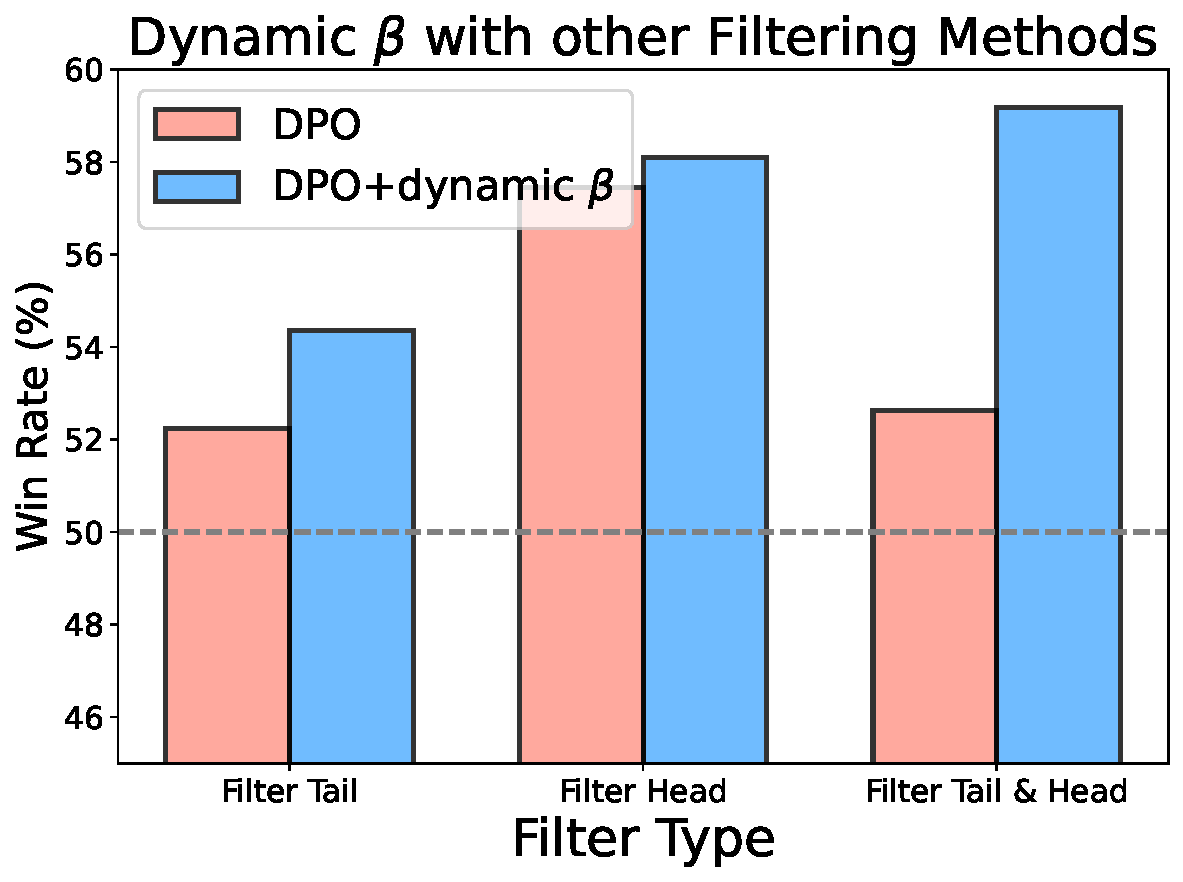
\includegraphics[width=0.4\textwidth]{figs/filter_gradient.pdf}
%     \includegraphics[width=0.4\textwidth]{figs/KTO-SPPO.pdf}
%     \caption{
%     \textbf{Left.} The win rates generated through GPT-4 evaluations for the Anthropic-HH single-turn dialogue reveal that $\beta$-DPO could adapt to various filtering strategies.
%     \textbf{Right.} The $\beta$-DPO approach win rates across different DPO variants, using GPT-4 as evaluator.}
%     % TL;DR summarization win rates vs. chosen summaries, using GPT-4 as evaluator; $\beta$-DPO emerges as the sole methodology attaining a win rate exceeding 50\% across various sampling temperatures.}
%     % \vspace{-2mm}
%     \label{fig:gradient}
% \end{figure}

\begin{figure}
    \centering
    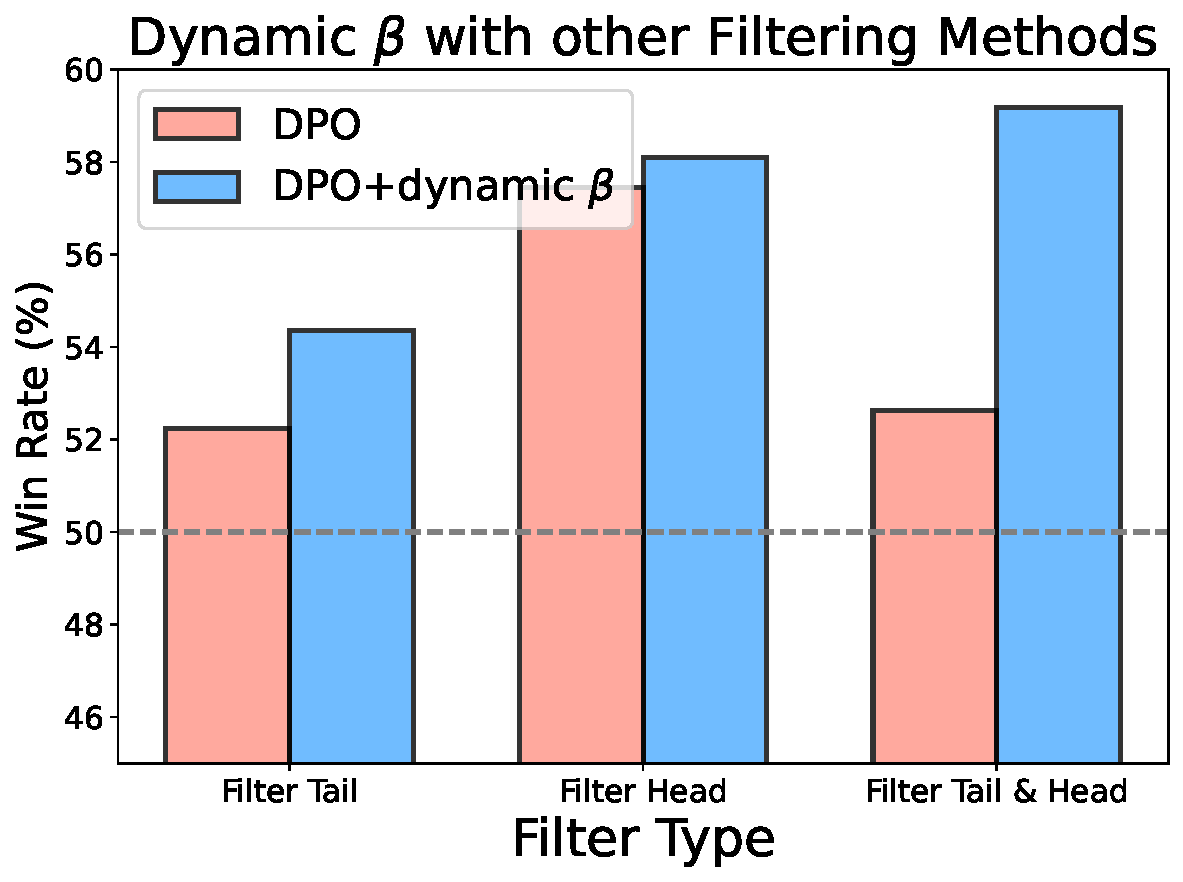
\includegraphics[width=0.32\textwidth]{figs/filter_gradient.pdf}
    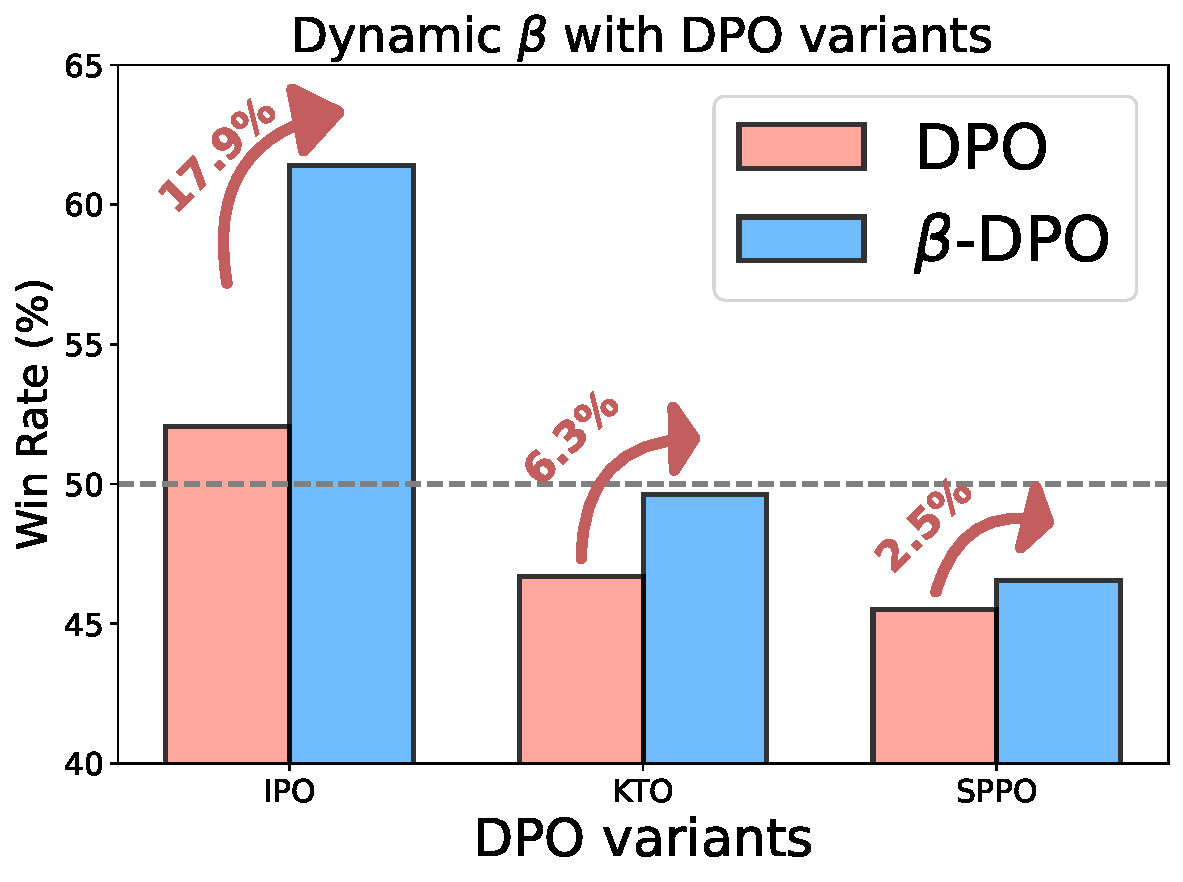
\includegraphics[width=0.32\textwidth]{figs/kto-sppo.pdf}
    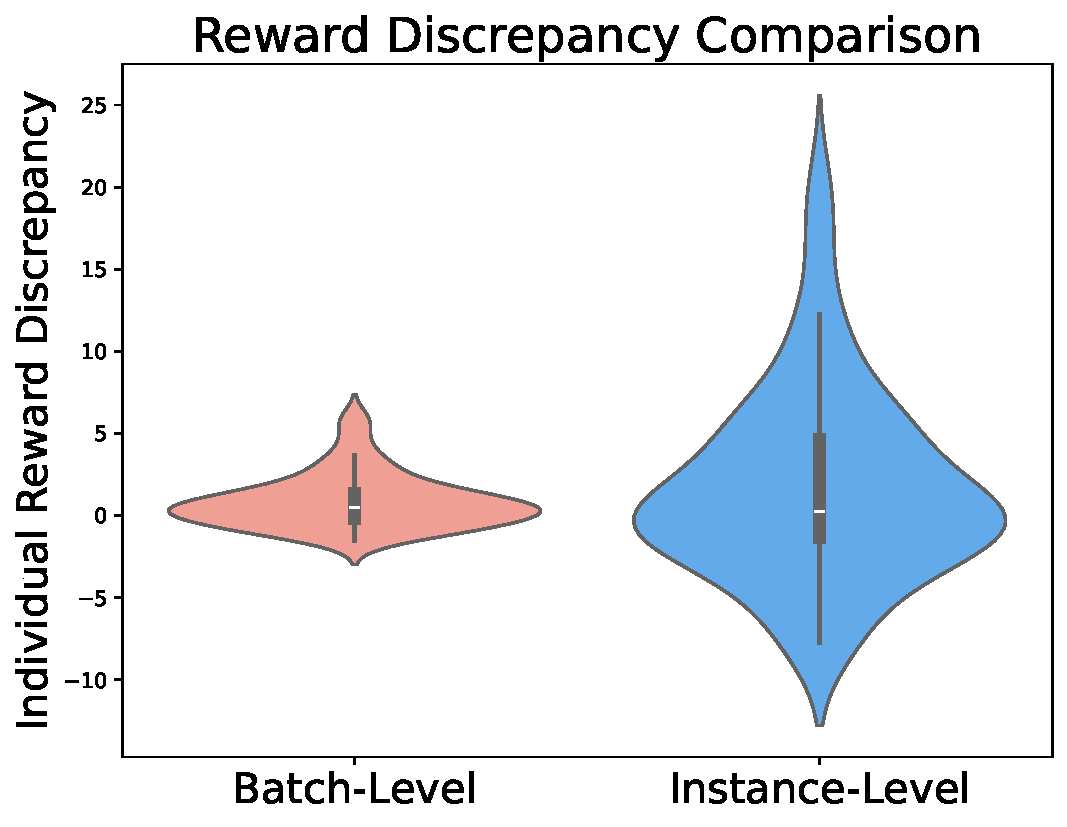
\includegraphics[width=0.32\textwidth]{figs/gap_batch_instance.pdf}
    \caption{
    \textbf{Left:} Win rates from GPT-4 evaluations on Anthropic-HH single-turn dialogues, showcasing $\beta$-DPO's adaptability to diverse filtering strategies. \textbf{Middle:} Win rates of $\beta$-DPO across various DPO variants as evaluated by GPT-4. \textbf{Right:} Distribution of individual reward discrepancies following fine-tuning through batch-level and instance-level calibration.
    % \textbf{Left:} The win rates generated through GPT-4 evaluations for the Anthropic-HH single-turn dialogue reveal that $\beta$-DPO could adapt to various filtering strategies.
    % \textbf{Middle:} The $\beta$-DPO approach win rates across different DPO variants, using GPT-4 as evaluator.
    % \textbf{Right:} The distribution of individual reward discrency after fined-tuned by batch-level calibration and instance-level calibration.
    }
    
    % TL;DR summarization win rates vs. chosen summaries, using GPT-4 as evaluator; $\beta$-DPO emerges as the sole methodology attaining a win rate exceeding 50\% across various sampling temperatures.}
    % \vspace{-2mm}
    \label{fig:gradient}
\end{figure}


\subsection{Necessity of Batch-Level Dynamic $\beta$ Calibration}
\label{sec_batch_level}
In this section, we aim to underscore the pivotal role of batch-level tuning in calibrating the parameter $\beta$. To this end, we compare the performance of our $\beta$-DPO algorithm under two distinct regimes: one employing batch-level dynamic $\beta$ calibration, and the other utilizing instance-level dynamics. To emulate the diverse data disparity scenarios encountered in practical applications, we adopt the methodology outlined in Section \ref{motivation_sec}, meticulously blending datasets characterized by both \emph{low gap} and \emph{high gap} attributes at varying ratios.

\textbf{Batch-level calibration surpasses both instance-level and population-level approaches.} The results presented in Table \ref{tab:noise} illustrate that batch-level dynamic $\beta$ calibration yields superior performance compared to instance-level dynamics and the baseline population-level approach (referred to as vanilla DPO) across a range of mixture ratios. This improvement can be credited to the batch-level calibration's ability to adjust to the varying data quality present within a batch, thus refining the model's learning process.
Conversely, instance-level dynamics can provoke excessively vigorous model updates, precipitating a decline in performance particularly noticeable at a mixture ratio of 40\%, a scenario in which outliers exert a significant negative impact.

\textbf{Instance-level calibration magnifies the impact of outliers.}
As demonstrated in Figure \ref{fig:gradient} (Right), instance-level calibration can inadvertently widen the range of reward discrepancy distribution. This broadened range suggests that instance-level calibration might be leading to excessively high or low $\beta$ values for the model. Such disparities in $\beta$ values consequently cause disproportionate update rates for certain samples, further intensifying the extremities in the distribution. 
\begin{table}
    \centering
    \caption{
    Comparison of win rates across varying mixture ratios on the Anthropic HH dataset, with each ratio indicating the proportion of \emph{high-gap} to \emph{low-gap} datasets, e.g., a 40\% mixture ratio reflects a blend of 40\% \emph{high-gap} and 60\% \emph{low-gap}.
    }
    \begin{tabular}{l|l|l|l|l}
        \toprule
        \textbf{Mixture Ratio} & \textbf{10\%} & \textbf{20\%} & \textbf{30\%} & \textbf{40\%}\\
        \midrule
        Vanilla DPO & $50.17$ & $50.56$ & $47.95$ & $29.15$ \\
        + Instance-level calibration & $49.18^{\color{-}- 1.97\%}$ & $49.82^{\color{-}- 1.46\%}$ & $44.42^{\color{-}- 7.36\%}$ & $16.82^{\color{-}- 42.30\%}$ \\
        + Batch-level calibration & $57.68^{\color{+}+ 14.69\%}$ & $56.15^{\color{+}+ 11.06\%}$ & $51.25^{\color{+}+ 6.88\%}$ & $34.92^{\color{+}+ 19.79\%}$ \\
        \bottomrule
    \end{tabular}
    \label{tab:noise}
\end{table}

% \setlength{\tabcolsep}{6pt}

\textbf{Our $\beta$-calibration strategy consistently outperforms baseline methods.} To expand our approach to more diverse datasets and model sizes, we follow the current state-of-the-art models SimPO \cite{SimPO2024}. We perform $\beta$-DPO with two families of models, Llama3-8B \citep{llama3modelcard}, Mistral2-7B \citep{Jiang2023Mistral7}, on the \href{https://huggingface.co/datasets/HuggingFaceH4/ultrachat_200k}{UltraChat-200k} dataset~\cite{Ding2023EnhancingCL}. For comparison with baselines, we assess our models using one of the most popular open-ended instruction-following benchmarks: AlpacaEval 2. All settings are consistent with SimPO \cite{SimPO2024}.
\begin{wraptable}[11]{r}{7.7cm}
\centering
\vspace{-0.6em}
\caption{Performance comparison of different models}
 \small
\resizebox{7.7cm}{!}{
\begin{tabular}{ccccc}
\toprule
\multirow{2}{*}{Model} & \multicolumn{2}{c}{Mistral-Instruct (7B)} & \multicolumn{2}{c}{Llama3-Instruct (8B)} \\
\cmidrule(lr){2-3} \cmidrule(lr){4-5}
 & LC (\%) & WR (\%) & LC (\%) & WR (\%) \\
\midrule
DPO & 20.98 & \textbf{21.60} & 40.44 & 37.38 \\
$\beta$-DPO & \textbf{23.56} & 20.42 & \textbf{43.38} & \textbf{38.21} \\
\midrule
SimPO & 28.50 & 30.56 & 44.38 & 38.97 \\
$\beta$-SimPO & \textbf{30.48} & \textbf{32.13} & \textbf{46.03} & \textbf{40.18} \\
\bottomrule
\end{tabular}
}
\label{tab:performance_comparison_lc}
\end{wraptable}
Table \ref{tab:performance_comparison_lc} presents the AlpacaEval 2 results under the Mistral-Instruct (7B) and Llama3-Instruct (8B) settings. LC and WR denote length-controlled and raw win rate, respectively. Regardless of whether we use Llama3-8B or Mistral-7B, and whether the loss function is DPO or SimPO, our $\beta$-{D, Sim}PO strategy consistently demonstrates significant performance improvements. This thoroughly showcases the method's strong generalization ability and excellent scalability.
% \begin{table}[h!]
% \centering
% \begin{tabular}{ccccccccccc}
% \hline
% % Method & DPO & $\beta$-DPO  & SimPO  & $\beta$-SimPO & SimPO & $\beta$-SimPO & $\beta$-SimPO & SimPO & $\beta$-SimPO & $\beta$-SimPO  \\
% % RM &implicit & implicit &implicit & implicit & PairRM & PairRM & PairRM & ArmoRM &ArmoRM &ArmoRM \\
% &BL & BL &BL & BL & BL & IL & BL & BL & IL & BL\\
% \hline
% LC (\%) & 40.44 & \textbf{43.38} & 44.38 & \textbf{46.03} & 44.7 & 43.84 & \textbf{45.65} & 53.7 & 49.05 & \textbf{54.86} \\
% \hline
% WR (\%) & 37.38 & \textbf{38.21} & 38.97 & \textbf{40.18} & 38.98 & 38.54 & \textbf{39.76} & 47.50 & 45.47 & \textbf{49.66} \\
% \hline
% \end{tabular}
% \caption{Performance comparison of different methods}
% \label{tab:performance_comparison}
% \end{table}

